\chapter{CÁC LUỒNG DỮ LIỆU CHÍNH CỦA HỆ THỐNG}

Phần này tổng hợp các luồng dữ liệu quan trọng nhất trong toàn bộ hệ thống, từ luồng hỏi đáp trực tiếp qua Rasa, luồng chuyển nhánh sang RAG, đến các luồng quản trị như huấn luyện mô hình, quản lý dữ liệu huấn luyện, ingest tài liệu và phân quyền RBAC. Mỗi luồng được mô tả theo hai góc nhìn: góc nhìn nghiệp vụ thể hiện trên sơ đồ sequence, và góc nhìn triển khai dựa trên mã nguồn của frontend, Flask API, Rasa và KmaRAG.

\section{Luồng chat thường qua Rasa}

Luồng này mô tả trường hợp người dùng gửi một câu hỏi thông thường và hệ thống có thể xử lý trọn vẹn trong nhánh Rasa mà không cần chuyển sang RAG. Dữ liệu đi từ giao diện chat ở frontend, qua lớp Flask API trung gian, sau đó được chuyển tới Rasa để phân loại ý định, chọn rule hoặc action phù hợp và trả phản hồi về cho người dùng.

\begin{figure}[H]
    \centering
    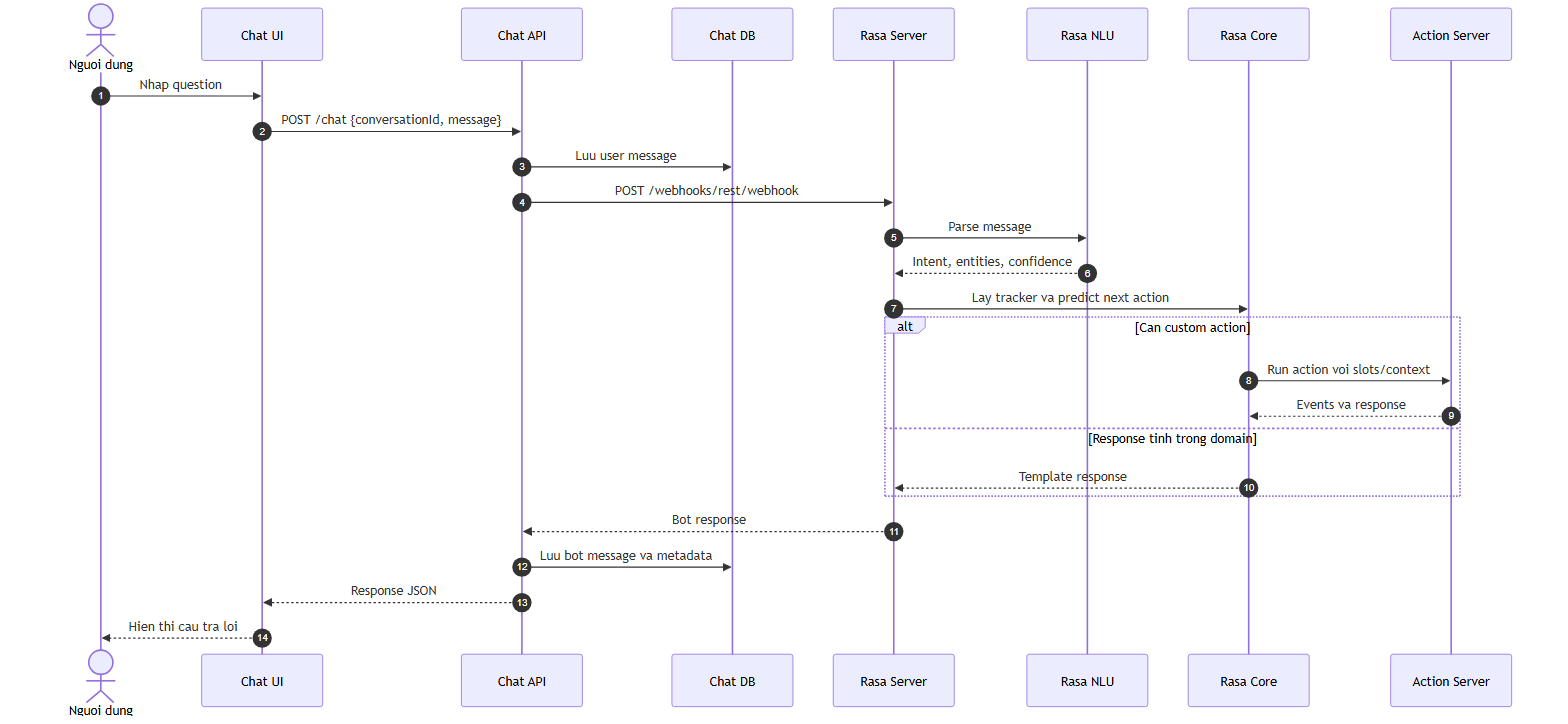
\includegraphics[width=\textwidth]{content/source/mermaid_sequence/seq_01.png}
    \caption{Luồng chat thường qua Rasa}
\end{figure}

Về mặt xử lý, frontend đóng vai trò thu thập nội dung câu hỏi và gắn với chatbot đang được chọn hoặc phiên hội thoại hiện tại. Flask API chuẩn hóa request, chuyển tiếp sang webhook REST của Rasa, sau đó gom các message phản hồi thành dữ liệu trả về cho giao diện. Trong Rasa, pipeline NLU nhận diện intent, entity và kích hoạt tầng quản lý hội thoại để suy ra response hoặc action tiếp theo. Khi intent có độ tin cậy đủ cao và rule tương ứng đã được định nghĩa, câu trả lời được tạo ra hoàn toàn trong nhánh này.

\section{Luồng chat stream có phân nhánh Rasa/RAG và fallback RAG}

Luồng này mô tả trường hợp hệ thống hỗ trợ trả lời theo chế độ stream, đồng thời có thể phân nhánh giữa xử lý bằng Rasa và xử lý bằng RAG. Đây là luồng quan trọng nhất đối với các câu hỏi tự nhiên, vì nó cho thấy cách hệ thống kết hợp rule-based dialogue với truy xuất tri thức từ kho tài liệu.

\begin{figure}[H]
    \centering
    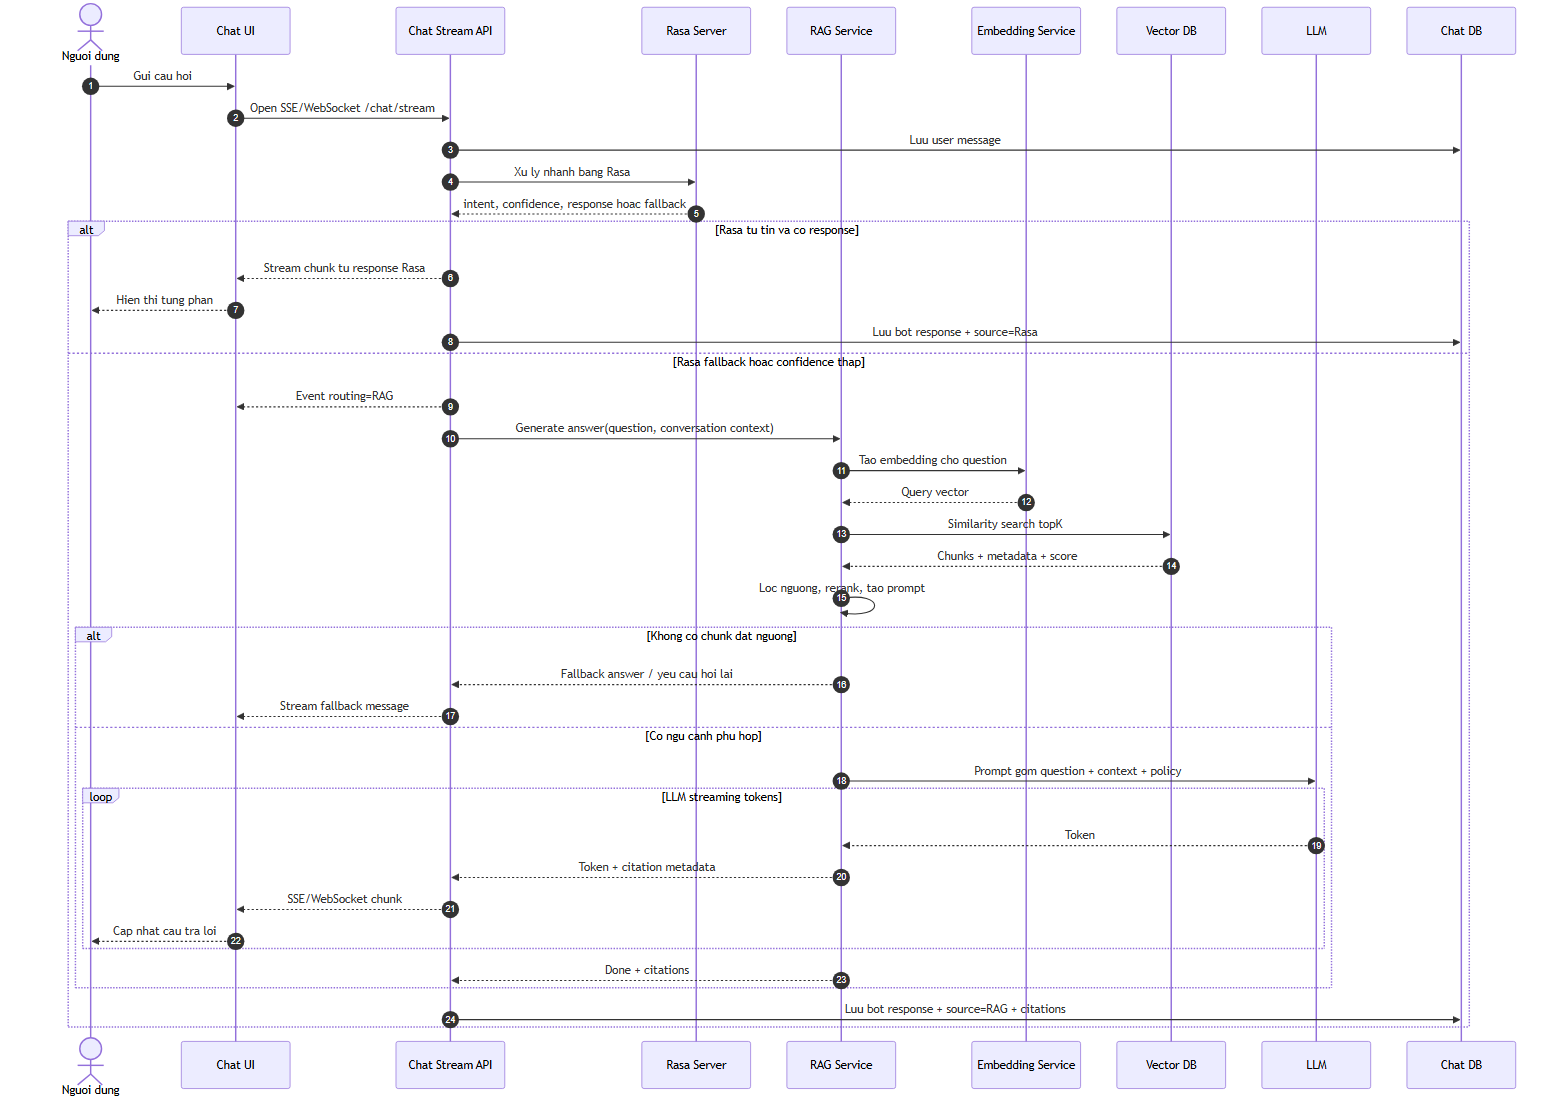
\includegraphics[width=\textwidth]{content/source/mermaid_sequence/seq_02.png}
    \caption{Luồng chat stream có phân nhánh Rasa/RAG và fallback RAG}
\end{figure}

Ở pha đầu, người dùng gửi câu hỏi và frontend mở kết nối nhận phản hồi theo dòng. Flask API đóng vai trò điều phối: nếu intent trong Rasa đủ tin cậy thì phản hồi đi theo nhánh hội thoại thông thường; nếu rơi vào \path{nlu_fallback}, action của Rasa sẽ gọi sang KmaRAG để truy xuất ngữ cảnh, dựng prompt và sinh câu trả lời. Nhờ cơ chế stream, câu trả lời có thể được đẩy dần về giao diện thay vì chờ hoàn tất toàn bộ. Kiến trúc này giữ được tốc độ xử lý cho câu hỏi phổ biến, đồng thời vẫn hỗ trợ câu hỏi dài hoặc phụ thuộc vào tài liệu.

\section{Luồng upload/run model}

Luồng này mô tả quy trình đưa một mô hình Rasa mới vào hệ thống và kích hoạt mô hình đó để phục vụ chatbot. Đây là luồng quản trị vận hành, thường được sử dụng khi đã có mô hình huấn luyện sẵn và cần cập nhật môi trường chạy mà không phải sửa trực tiếp trong mã nguồn ứng dụng.

\begin{figure}[H]
    \centering
    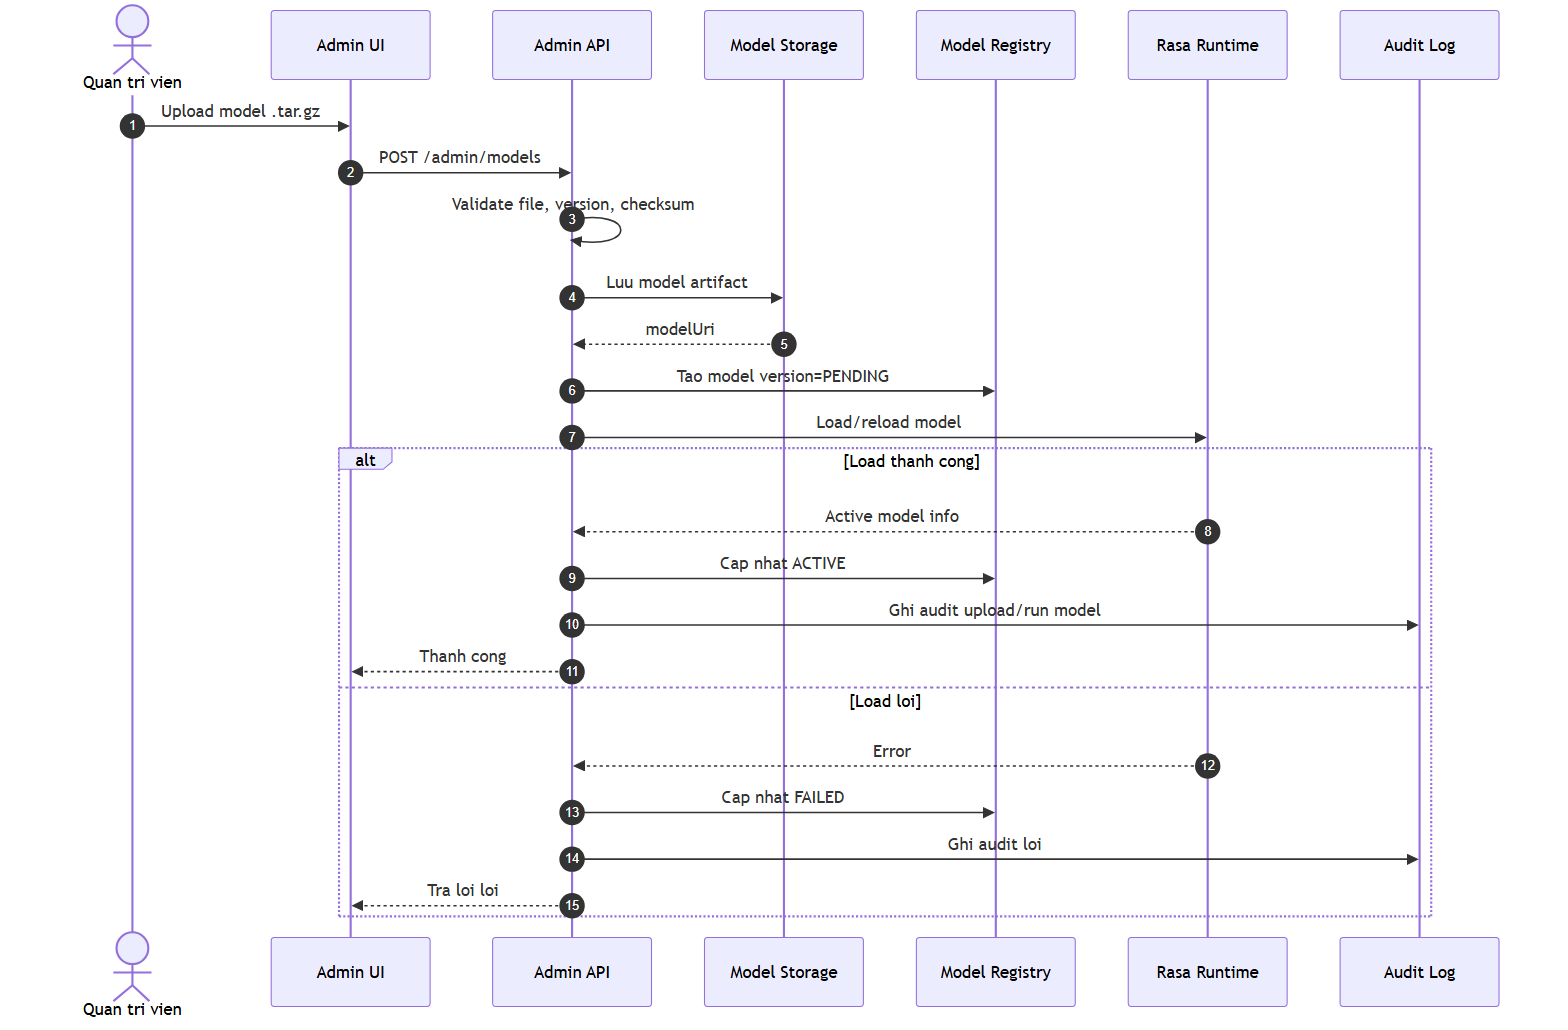
\includegraphics[width=\textwidth]{content/source/mermaid_sequence/seq_03.png}
    \caption{Luồng upload/run model}
\end{figure}

Theo sequence, người quản trị chọn mô hình hoặc gói mô hình trên giao diện, frontend tải tệp lên backend quản trị, sau đó backend lưu mô hình, cập nhật metadata và yêu cầu Rasa nạp mô hình tương ứng. Sau khi thao tác hoàn tất, trạng thái mô hình đang chạy được phản hồi trở lại để giao diện hiển thị kết quả. Luồng này tách riêng bước quản lý tệp mô hình và bước kích hoạt runtime, nhờ đó hệ thống có thể kiểm soát lịch sử mô hình tốt hơn.

\section{Luồng push/run actions}

Luồng này mô tả quy trình cập nhật mã custom actions và đưa action server vào trạng thái chạy sẵn sàng phục vụ Rasa. Trong hệ thống, nhánh này đặc biệt quan trọng vì nhiều hành vi nghiệp vụ như gọi RAG, tra cứu tài liệu, ghi log câu hỏi chưa xử lý tốt hay trích xuất thông tin đều đi qua custom action thay vì response tĩnh.

\begin{figure}[H]
    \centering
    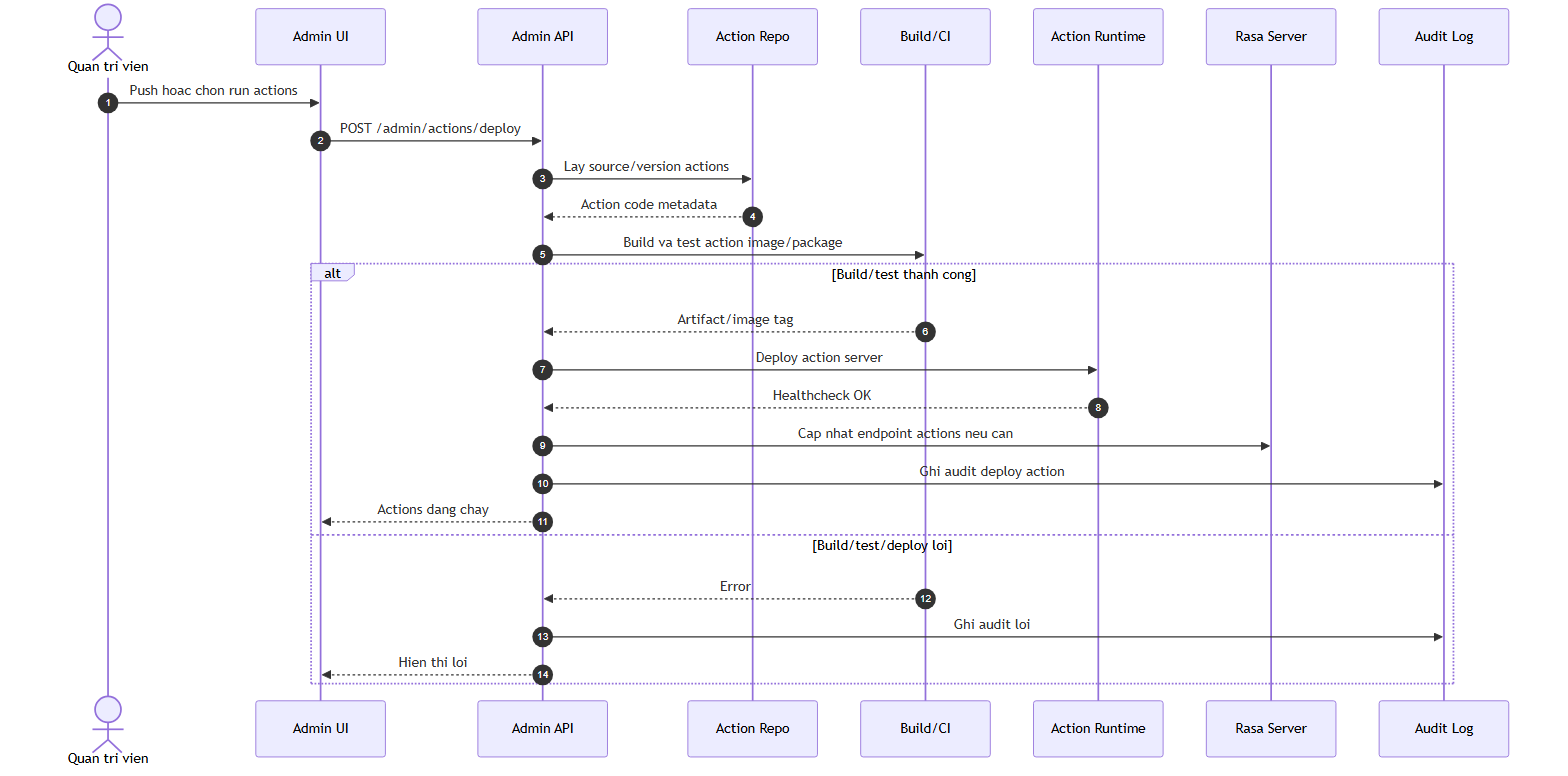
\includegraphics[width=\textwidth]{content/source/mermaid_sequence/seq_04.png}
    \caption{Luồng push/run actions}
\end{figure}

Về nghiệp vụ, quản trị viên cập nhật mã action hoặc lựa chọn action cần triển khai, hệ thống chuyển mã hoặc cấu hình mới tới backend, sau đó khởi động lại hoặc nạp lại action server để Rasa có thể gọi các action tương ứng. Sau khi action server chạy ổn định, chatbot mới có thể thực thi các bước nghiệp vụ cần truy cập dữ liệu bên ngoài hoặc tích hợp với KmaRAG.

\section{Luồng quản lý intent/entity/response/rule/story/action}

Luồng này mô tả nhóm thao tác quản trị cấu hình tri thức hội thoại của chatbot, bao gồm intent, entity, response, rule, story và action. Đây là luồng quản lý cốt lõi để duy trì khả năng hiểu câu hỏi, tổ chức phản hồi và kiểm soát logic hội thoại của Rasa theo thời gian.

\begin{figure}[H]
    \centering
    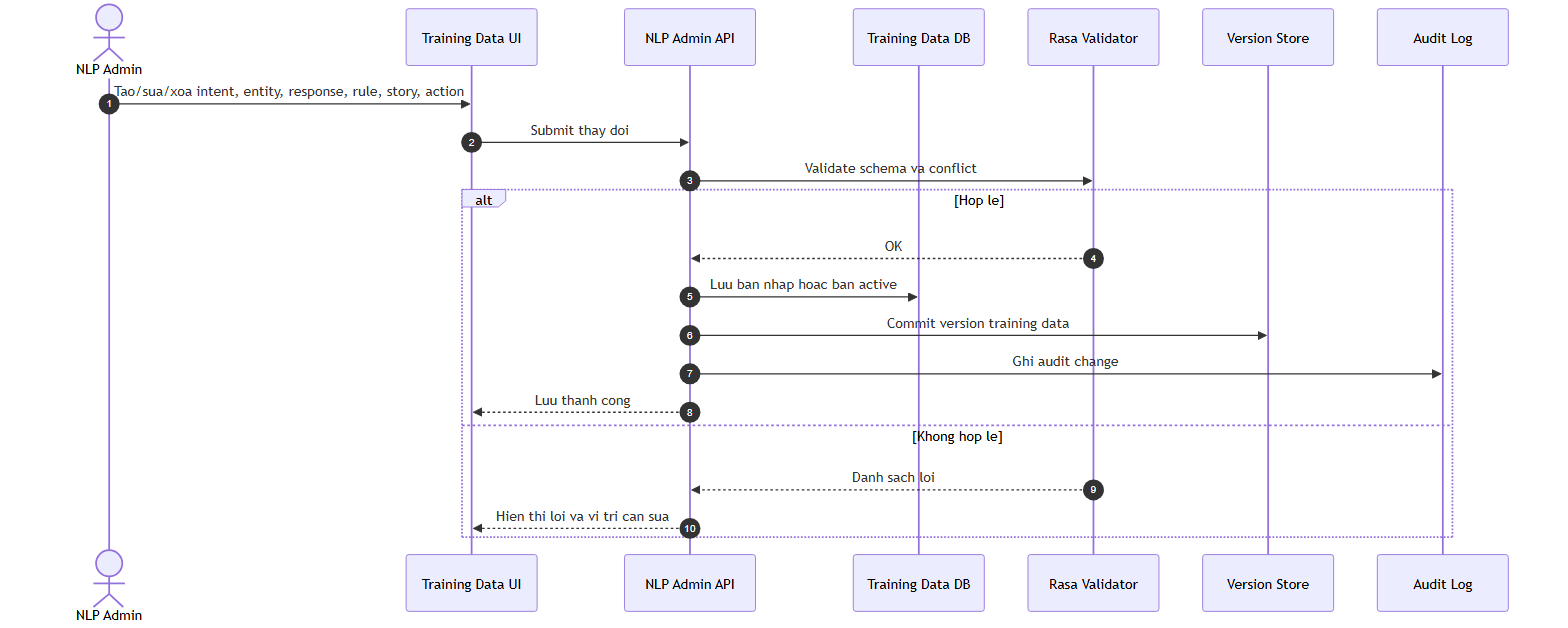
\includegraphics[width=\textwidth]{content/source/mermaid_sequence/seq_05.png}
    \caption{Luồng quản lý intent/entity/response/rule/story/action}
\end{figure}

Theo sequence, người quản trị tạo mới, cập nhật hoặc xóa các phần tử hội thoại trên giao diện; dữ liệu được gửi tới backend quản trị thông qua các API riêng cho từng loại đối tượng; backend xác thực, lưu trữ, rồi đồng bộ trở lại trạng thái mới cho frontend. Luồng này không chỉ phục vụ việc nhập dữ liệu NLU mà còn là cơ sở để tạo rule, story và response phục vụ suy diễn hội thoại trong Rasa.

\section{Luồng active training data và train model}

Luồng này mô tả quy trình tận dụng dữ liệu phản hồi thực tế hoặc dữ liệu được quản trị viên chuẩn hóa để bổ sung vào tập huấn luyện, sau đó kích hoạt huấn luyện mô hình mới. Đây là chu trình cải tiến liên tục, giúp chatbot thích nghi với câu hỏi mới và nâng độ chính xác của phân loại intent cũng như điều phối hội thoại.

\begin{figure}[H]
    \centering
    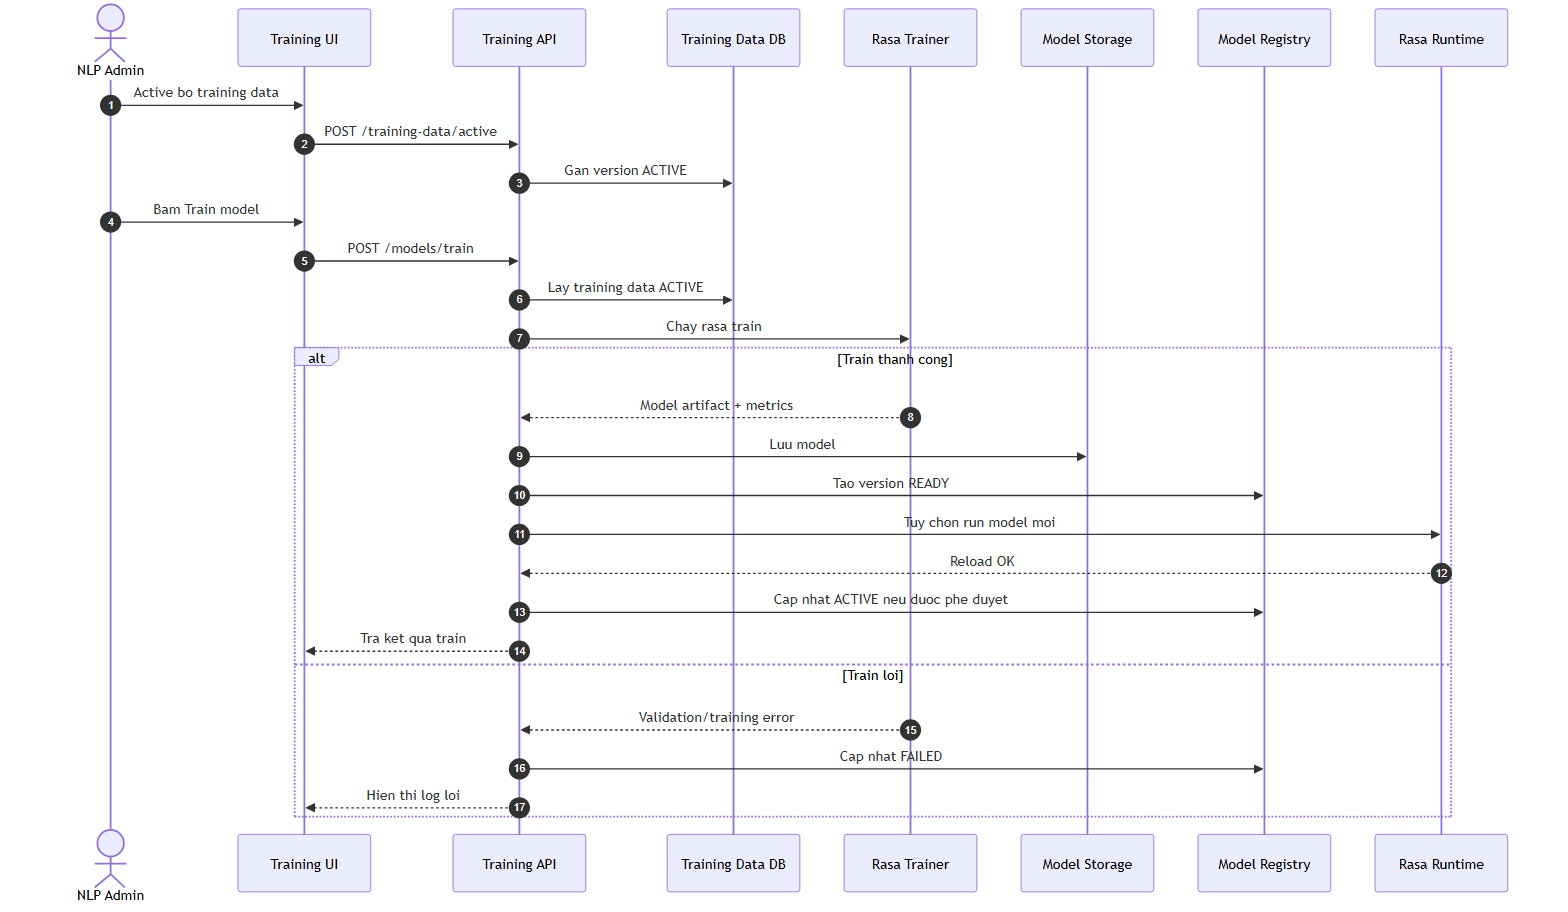
\includegraphics[width=\textwidth]{content/source/mermaid_sequence/seq_06.png}
    \caption{Luồng active training data và train model}
\end{figure}

Về nghiệp vụ, dữ liệu huấn luyện được duyệt hoặc chọn từ giao diện quản trị, chuyển tới backend để tổng hợp cùng intent, entity, rule và story hiện hành, sau đó hệ thống gọi tiến trình train model. Khi quá trình train hoàn tất, metadata về mô hình mới được lưu lại và giao diện có thể tiếp tục sử dụng luồng upload/run model để đưa mô hình vào vận hành. Sequence này thể hiện rõ chu trình dữ liệu từ quan sát thực tế đến cải tiến mô hình.

\section{Luồng ghi nhận câu hỏi chưa xử lý tốt}

Luồng này mô tả cơ chế hệ thống ghi lại các câu hỏi mà chatbot chưa xử lý tốt, bao gồm trường hợp không nhận diện được intent, trả lời chưa đúng trọng tâm hoặc phải rơi vào fallback nhiều lần. Đây là đầu vào rất quan trọng cho quy trình active training và cải thiện chất lượng hội thoại.

\begin{figure}[H]
    \centering
    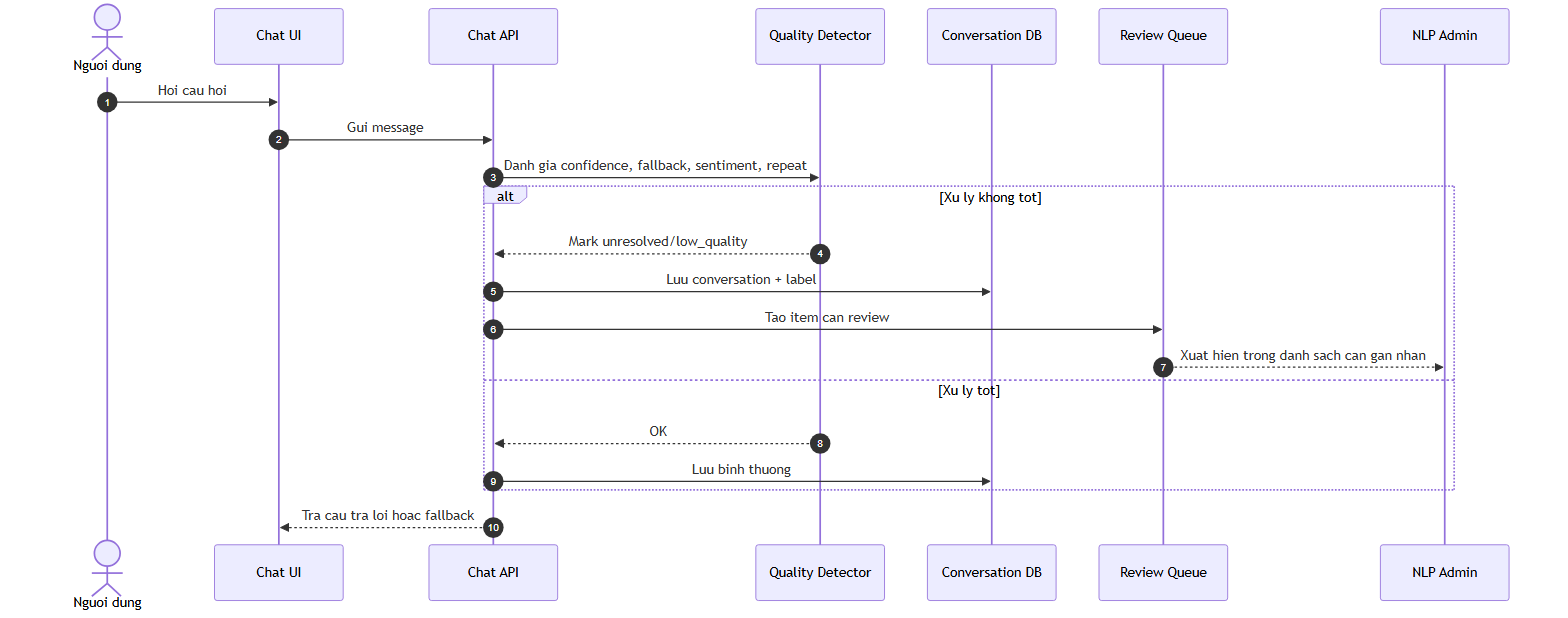
\includegraphics[width=\textwidth]{content/source/mermaid_sequence/seq_07.png}
    \caption{Luồng ghi nhận câu hỏi chưa xử lý tốt}
\end{figure}

Về mặt dữ liệu, sau khi một lượt hội thoại kết thúc hoặc bị đánh giá là chưa đạt, hệ thống tạo bản ghi chứa câu hỏi, ngữ cảnh liên quan, trạng thái xử lý và thông tin phản hồi của người dùng hoặc quản trị viên. Dữ liệu này được chuyển về khu vực quản trị để người vận hành xem xét, gán nhãn hoặc chuyển hóa thành ví dụ huấn luyện mới. Nhờ đó, các câu hỏi thực tế từ người dùng không bị thất thoát mà trở thành nguồn cải tiến hệ thống.

\section{Luồng ingest tài liệu RAG}

Luồng ingest tài liệu RAG mô tả cách hệ thống tiếp nhận tài liệu ngữ cảnh, lưu vào kho tài liệu, tiền xử lý, cắt đoạn, lập chỉ mục và đưa dữ liệu vào tầng truy xuất của KmaRAG. Đây là luồng nền tảng để các câu hỏi cần tài liệu có thể được RAG hỗ trợ chính xác và có dẫn nguồn.

\begin{figure}[H]
    \centering
    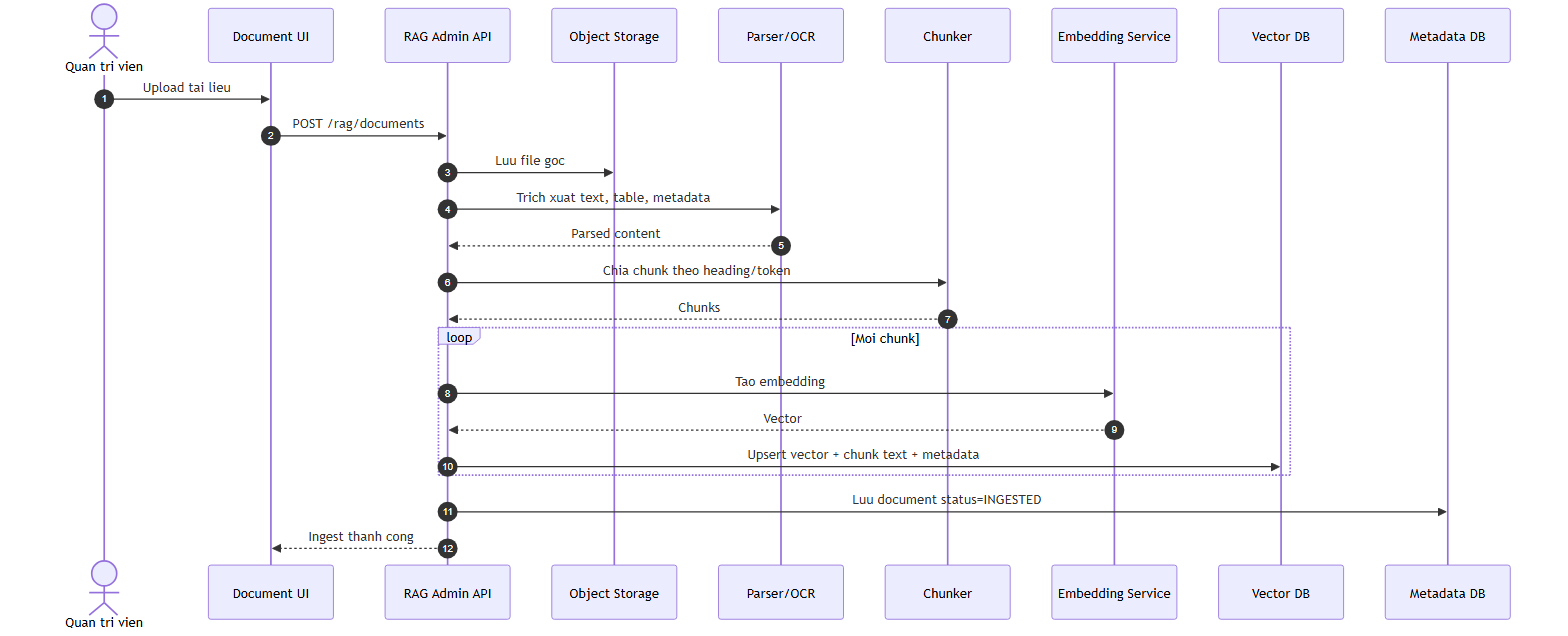
\includegraphics[width=\textwidth]{content/source/mermaid_sequence/seq_08.png}
    \caption{Luồng ingest tài liệu RAG}
\end{figure}

Theo sequence, quản trị viên tải tài liệu lên từ giao diện, backend nhận tệp, quét an toàn tên tệp, lưu tài liệu vào vùng nhập, sau đó khởi tạo pipeline xử lý nền. Trong pipeline này, tài liệu được chuyển sang văn bản sạch, phân đoạn, sinh embedding và cập nhật các kho lưu trữ cần thiết như vector store, document metadata hoặc graph. Sau khi ingest hoàn tất, tài liệu trở thành một phần của kho tri thức mà nhánh query có thể truy xuất.

\section{Luồng phân quyền RBAC}

Luồng RBAC mô tả cách hệ thống kiểm soát truy cập theo vai trò và quyền hạn. Đây là luồng quản trị bắt buộc vì hệ thống đồng thời có người dùng cuối, quản trị viên nội dung và quản trị viên hệ thống; mỗi nhóm chỉ được thực hiện đúng các thao tác được cấp phép.

\begin{figure}[H]
    \centering
    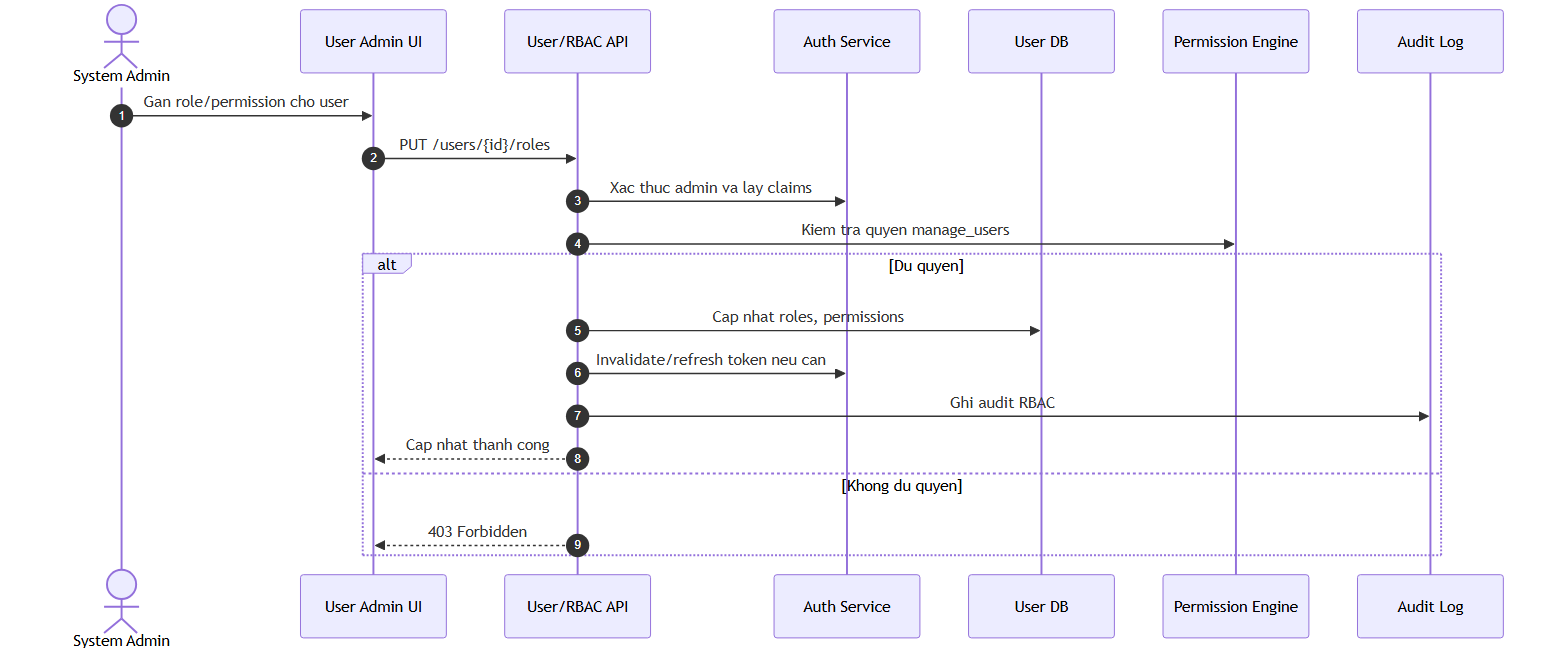
\includegraphics[width=\textwidth]{content/source/mermaid_sequence/seq_09.png}
    \caption{Luồng phân quyền RBAC}
\end{figure}

Theo sequence, quản trị viên tạo vai trò, định nghĩa quyền cho vai trò, gán vai trò vào người dùng và để frontend áp dụng kiểm tra quyền trước khi hiển thị hoặc kích hoạt chức năng. Khi người dùng gọi API, backend tiếp tục xác thực token, kiểm tra quyền trên tài nguyên và chỉ cho phép thao tác nếu vai trò tương ứng đáp ứng điều kiện. Cách thiết kế này bảo đảm vừa có lớp chặn ở giao diện, vừa có lớp kiểm soát thực sự ở backend.

\section{Luồng feedback câu trả lời để cải thiện chatbot}

Luồng feedback mô tả cách người dùng hoặc quản trị viên đánh giá chất lượng một câu trả lời, từ đó tạo ra dữ liệu đầu vào cho việc hiệu chỉnh rule, intent hoặc tài liệu ngữ cảnh. Đây là luồng rất quan trọng đối với một hệ thống học hỏi từ vận hành thực tế, vì nó biến phản hồi người dùng thành dữ liệu cải tiến có cấu trúc.

\begin{figure}[H]
    \centering
    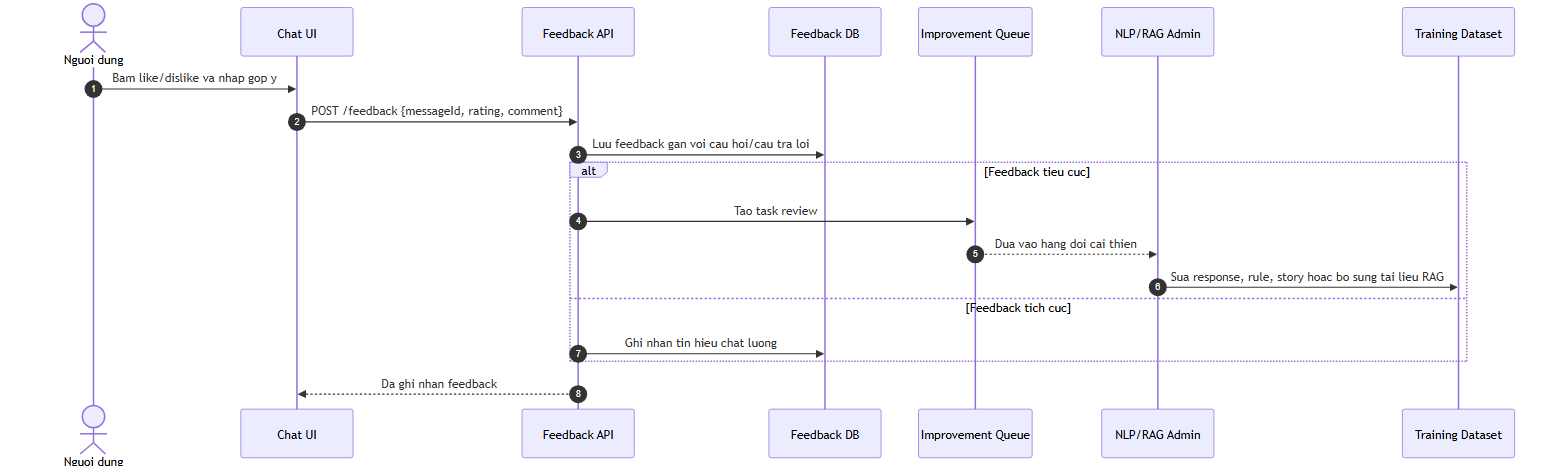
\includegraphics[width=\textwidth]{content/source/mermaid_sequence/seq_10.png}
    \caption{Luồng feedback câu trả lời để cải thiện chatbot}
\end{figure}

Về nghiệp vụ, sau khi chatbot trả lời, người dùng có thể đánh giá câu trả lời là phù hợp hoặc chưa phù hợp; thông tin này được gửi về backend và liên kết với câu hỏi, câu trả lời, ngữ cảnh hội thoại hoặc tài liệu tham chiếu đã sử dụng. Quản trị viên sau đó xem xét feedback, xác định nguyên nhân đến từ dữ liệu NLU, rule hội thoại hay truy xuất RAG, rồi cập nhật thành phần tương ứng. Luồng này là cầu nối giữa lớp sử dụng thực tế và lớp cải tiến chất lượng hệ thống.

\section{Luồng lưu lịch sử hội thoại}

Luồng này mô tả cách hệ thống lưu lại lịch sử trao đổi giữa người dùng và chatbot để phục vụ tra cứu lại cuộc hội thoại, thống kê, đánh giá chất lượng và làm giàu ngữ cảnh cho các xử lý tiếp theo. Đây là luồng dữ liệu hậu kỳ nhưng có giá trị lớn đối với cả trải nghiệm người dùng lẫn quản trị hệ thống.

\begin{figure}[H]
    \centering
    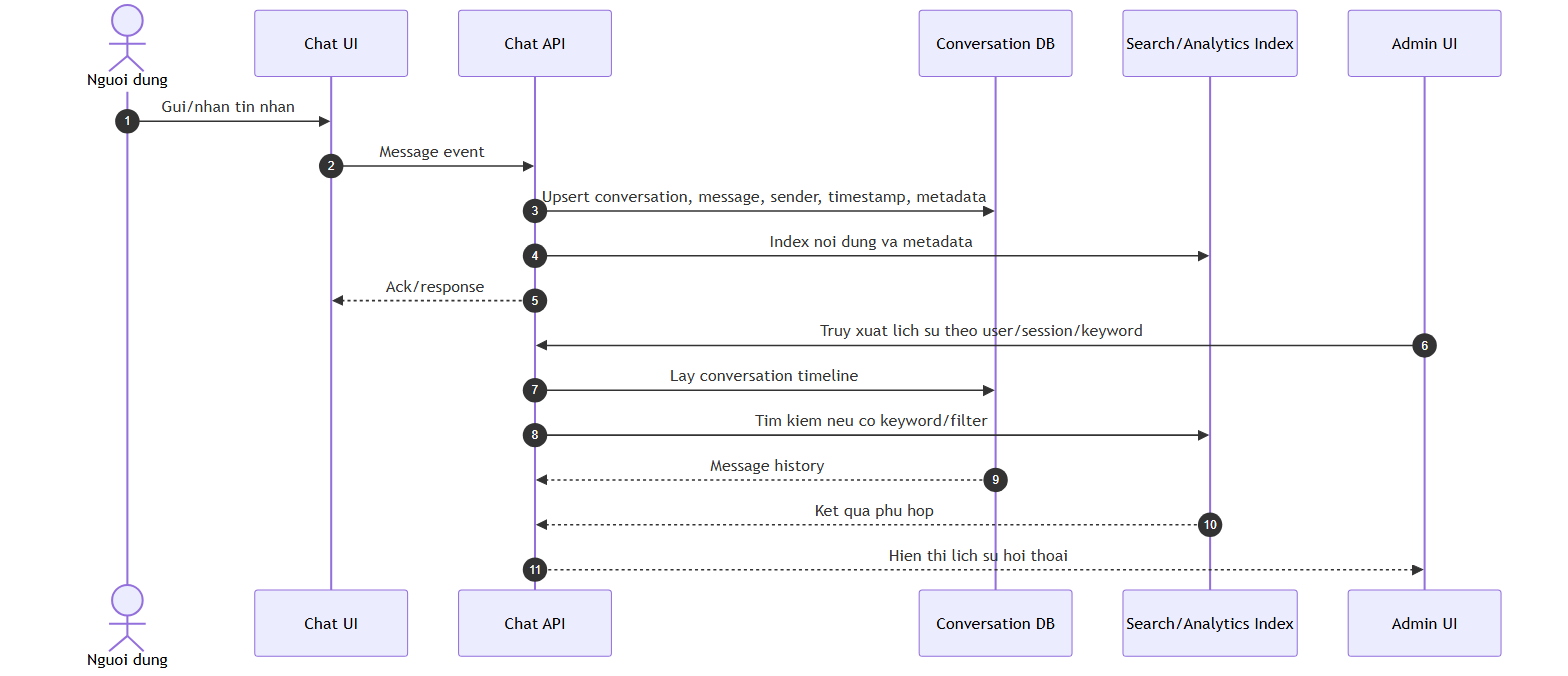
\includegraphics[width=\textwidth]{content/source/mermaid_sequence/seq_11.png}
    \caption{Luồng lưu lịch sử hội thoại}
\end{figure}

Theo sequence, sau khi người dùng gửi tin nhắn và chatbot trả phản hồi, backend ghép cặp các message thành một phần của phiên hội thoại và ghi chúng vào kho lưu trữ theo \path{conversationId}, \path{userId}, thời điểm tạo và cập nhật. Khi người dùng mở lại danh sách hội thoại hoặc xem chi tiết một cuộc trò chuyện, frontend gọi API lấy lịch sử để dựng lại toàn bộ ngữ cảnh đã có. Cơ chế này cũng giúp quản trị viên có dữ liệu để thống kê, kiểm thử hoặc truy nguyên khi xảy ra phản hồi bất thường.

